\chapter{Introduction}
\lhead{\chaptername~\thechapter. \emph{Introduction}}
The growing interest of the general public in spherical cameras technologies, which were 
research-only exclusives once, has made them less expensive and more available. For example, omindirectional cameras by GoPro have been extremely popular amongst sports men who publish them on social networks.

These devices have been employed in robotics since their first appearance to help navigate the robot in a real-world environment, and nowadays for autonomous driving. Furthermore, they can be exploited to deliver a virtual or augmented experience for augmented and virtual reality (AR/VR).

In this work, we designed a \textit{structure from motion} (SfM) pipeline for 
full spherical cameras. SfM is a well known topic in computer vision; it addresses the problem of 
recovering the structure of 3D environments from a sequence of images taken from different views.

SfM research (and computer vision in general) has targeted perspective cameras because these type of devices have always been more common. However, the increase of interest around these cameras has started a shift of interest towards employing them for research.

\section{Omnidirection Cameras}
Large field of view (FOV) photography employs fisheye lenses that are capable to cover 
wider scene compared to traditional cameras' hardware.
The applications for this kind of equipments range from architectural or 
landscape photography to academic use for studies related to astronomic, 
metereology, computer graphics, etc.
Photographers can also choose fisheye lenses for the characteristic distortion
they introduce that contributes to give more importance to foreground objects
(see Figure~\ref{fig:fisheye_example} for a wide FOV picture example).

\begin{figure}
	\centering
	\begin{subfigure}{0.4\textwidth}
		\centering
		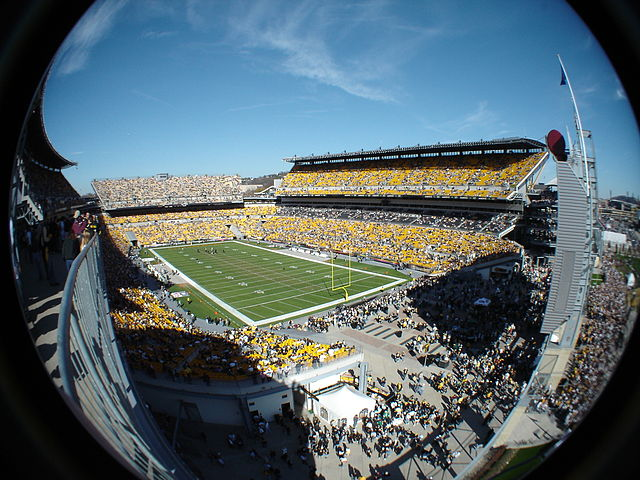
\includegraphics[width=0.7\textwidth]{img/fisheye_example}
		\caption{Fisheye.}\label{fig:fisheye_example}
	\end{subfigure}
	\begin{subfigure}{0.4\textwidth}
		\centering
		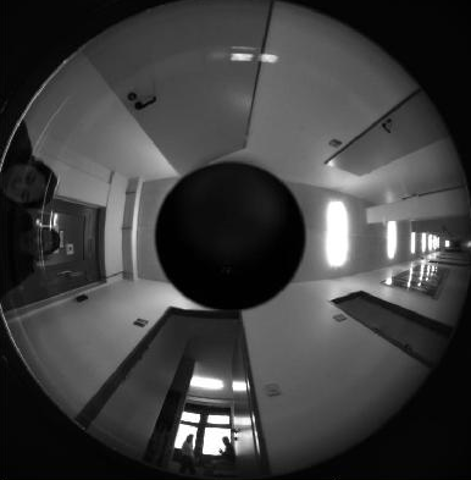
\includegraphics[width=0.7\textwidth]{img/omnidirectional_example}
		\caption{Ominidirectional (catadioptric).}\label{fig:omnidirectional_example}
	\end{subfigure}
	\caption{Some example of fisheye (\subref{fig:fisheye_example}) and omnidirectional (\subref{fig:omnidirectional_example}) pictures.}\label{fig:wide_fov_pics}
\end{figure}


\begin{figure}
	\centering
	\begin{subfigure}{0.3\textwidth}
		\centering
		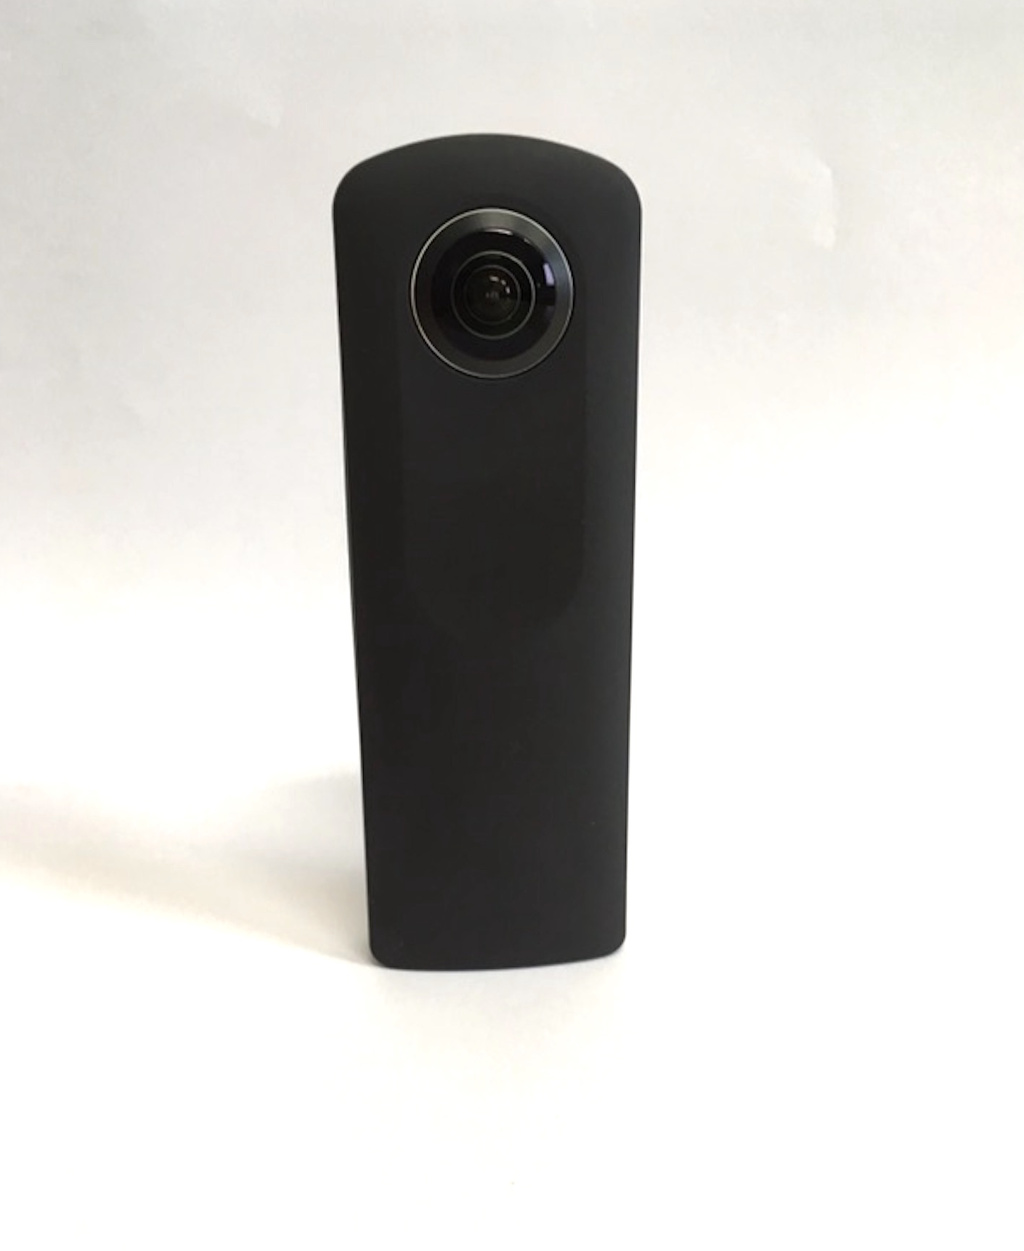
\includegraphics[width=0.7\textwidth]{img/theta1}
	\end{subfigure}
	\begin{subfigure}{0.3\textwidth}
		\centering
		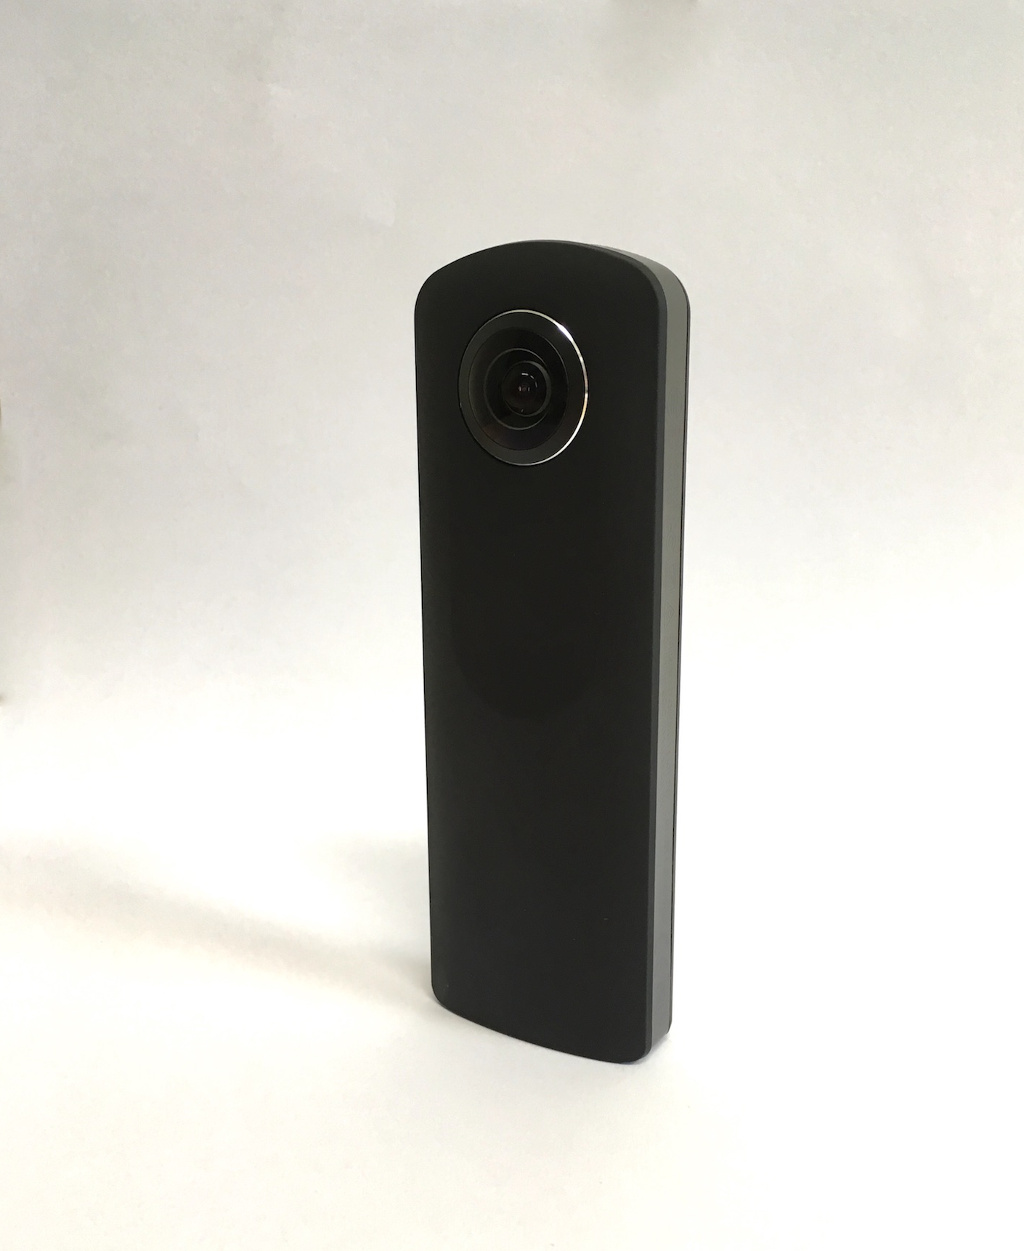
\includegraphics[width=0.7\textwidth]{img/theta2}
	\end{subfigure}
	\begin{subfigure}{0.3\textwidth}
		\centering
		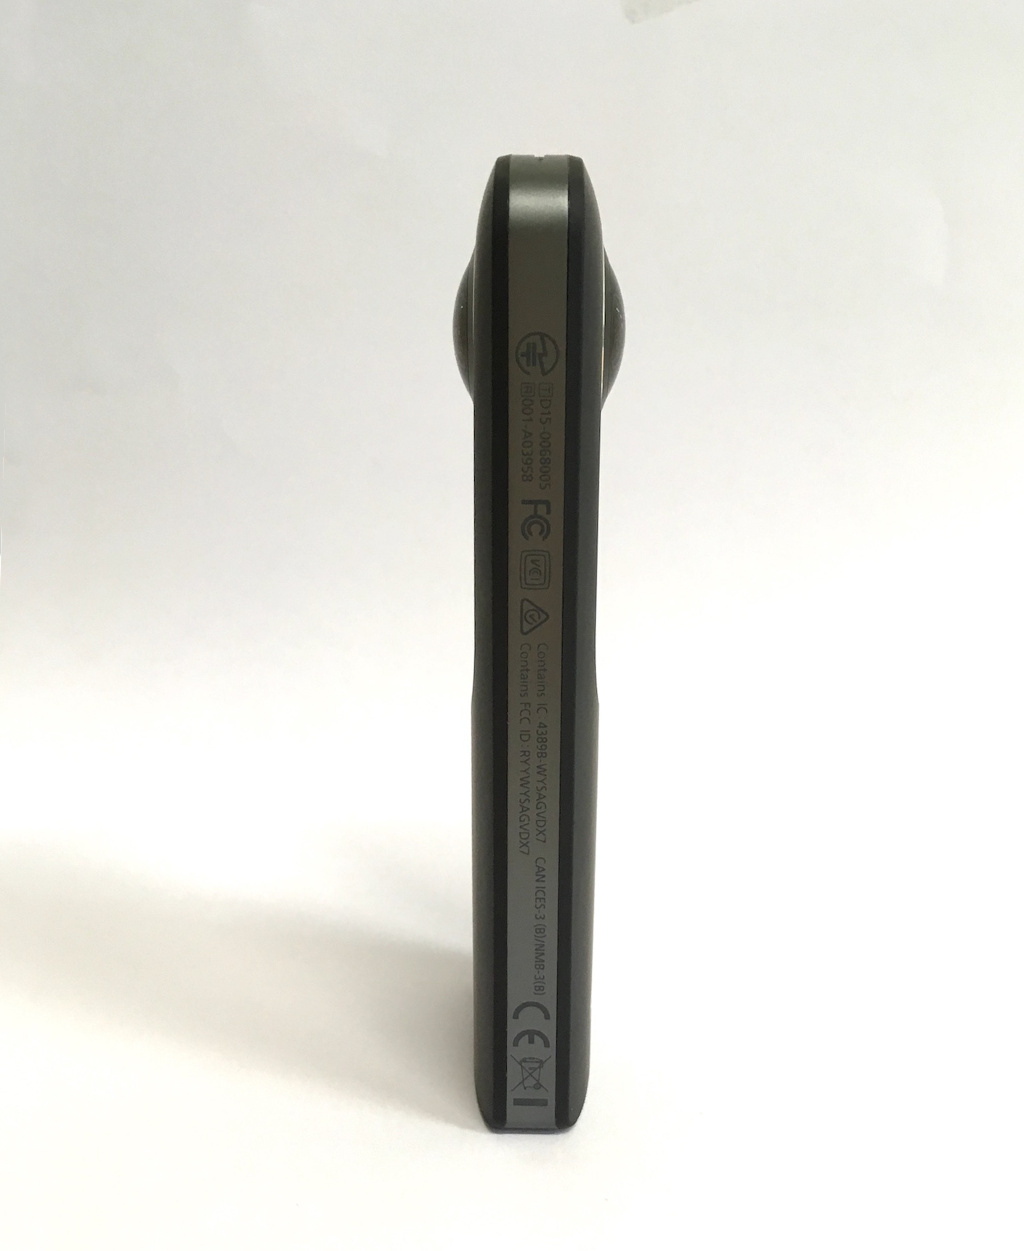
\includegraphics[width=0.7\textwidth]{img/theta3}
	\end{subfigure}
	\caption{\label{fig:ricoh_theta}The Ricoh Theta S 360\degree camera.}
\end{figure}
